\documentclass{article}
\usepackage[utf8]{inputenc}
\usepackage[T5]{fontenc}
\usepackage[fontsize=13pt]{scrextend}
\usepackage{multirow}
\usepackage[table,xcdraw]{xcolor}
\usepackage{pdflscape}
\usepackage{natbib}
\usepackage{listings}
\usepackage{array}
\usepackage[hyphens]{url}
\usepackage{xurl}
\usepackage[unicode]{hyperref}
\hypersetup{
    colorlinks=true,
    linkcolor=black,
    urlcolor=black,
    citecolor=black,
}
\urlstyle{same} % Đảm bảo toàn bộ URL và chuỗi ký tự hiển thị màu đen chuẩn

\lstset{
    basicstyle=\ttfamily\small,
    frame=single,
    breaklines=true,
    columns=fullflexible
}
\bibliographystyle{apalike}

\usepackage{longtable}
\usepackage[left=3cm, right=2.5cm, top=3cm, bottom=3cm]{geometry}
\usepackage{mathptmx} % Times New Roman
\usepackage{graphicx}
\usepackage{float}
\usepackage{wrapfig}
\usepackage{tikz}
\usetikzlibrary{calc}
\usepackage{indentfirst} % Thụt đầu dòng đoạn văn
\renewcommand{\baselinestretch}{1.2} % Giãn dòng 1.2
\setlength{\parskip}{6pt} % Khoảng cách giữa các đoạn
\setlength{\parindent}{1cm} % Khoảng cách thụt đầu dòng 1cm

\usepackage{titlesec}
\setcounter{secnumdepth}{4}

% Heading 1 - Section (Chương)
\titlespacing*{\section}{0pt}{12pt}{15pt}
\titleformat*{\section}{\fontsize{16pt}{0pt}\selectfont \bfseries \centering}

% Heading 2 - Subsection (2.2) - Lề trái 0pt
\titlespacing*{\subsection}{0pt}{8pt}{4pt}
\titleformat*{\subsection}{\fontsize{14pt}{0pt}\selectfont \bfseries}

% Heading 3 - Subsubsection (2.2.1) - Căn ngang hàng với 2.2 (Lề trái 0pt)
\titlespacing*{\subsubsection}{0pt}{6pt}{3pt}
\titleformat*{\subsubsection}{\fontsize{13pt}{0pt}\selectfont \bfseries \itshape}

% Heading 4 - Paragraph
\titlespacing*{\paragraph}{0pt}{4pt}{2pt}
\titleformat*{\paragraph}{\fontsize{13pt}{0pt}\selectfont \itshape}

\renewcommand{\figurename}{\fontsize{12pt}{0pt}\selectfont \bfseries Hình}
\renewcommand{\thefigure}{\thesection.\arabic{figure}}
\usepackage[font=bf]{caption}
\captionsetup[figure]{labelsep=space}

\renewcommand{\tablename}{\fontsize{12pt}{0pt}\selectfont \bfseries Bảng}
\renewcommand{\thetable}{\thesection.\arabic{table}}
\captionsetup[table]{labelsep=space}

\usepackage{tabularx}
\renewcommand{\theequation}{\thesection.\arabic{equation}}
\usepackage{colortbl}
\definecolor{LightCyan}{rgb}{0.88,1,1}

\renewcommand{\contentsname}{MỤC LỤC}
\renewcommand{\listfigurename}{DANH MỤC HÌNH VẼ}
\renewcommand{\listtablename}{DANH MỤC BẢNG BIỂU}
\renewcommand{\refname}{TÀI LIỆU THAM KHẢO}

% Khai báo thông tin dự án
\newcommand{\khoa}{CÔNG NGHỆ THÔNG TIN}
\newcommand{\mon}{DỰ ÁN CÔNG NGHỆ THÔNG TIN}
\newcommand{\de}{BÁO CÁO DỰ ÁN \\ BẢO MẬT HỒ SƠ Y TẾ BẰNG KIẾN TRÚC ZERO TRUST}
\newcommand{\gvhd}{TS. BÙI QUY ANH}
\newcommand{\svmot}{52300267 - Huỳnh Nguyễn Quốc Việt}
\newcommand{\svhai}{52300268 - Nguyễn Hoàng Việt}
\newcommand{\lop}{23050401}
\newcommand{\khoahoc}{27}
\newcommand{\nam}{2026}

\begin{document}

    \pagenumbering{gobble}
\begin{center}
	\fontsize{14pt}{0pt}\selectfont TỔNG LIÊN ĐOÀN LAO ĐỘNG VIỆT NAM \\
	\fontsize{14pt}{0pt}\selectfont \textbf{TRƯỜNG ĐẠI HỌC TÔN ĐỨC THẮNG} \\
	\fontsize{14pt}{0pt}\selectfont \textbf{KHOA \khoa} \\\vspace*{6pt}
	
\includegraphics[width=0.3\linewidth]{image/logo/tdtu.jpg}\\\vspace*{0.3cm}
 
	\fontsize{14pt}{0pt}\selectfont \textbf{Sinh viên thực hiện:}\\[4pt]
	\fontsize{14pt}{0pt}\selectfont \textbf{\svmot}\\[4pt]
	\fontsize{14pt}{0pt}\selectfont \textbf{\svhai}\\[1.5cm]

	\fontsize{22pt}{18pt}\selectfont \textbf{\de}\\\vspace*{2cm}
    
	\fontsize{18pt}{0pt}\selectfont \textbf{\mon}\vspace*{6pt}\\\vspace*{2cm}
 
	\fontsize{14pt}{0pt}\selectfont \textbf{THÀNH PHỐ HỒ CHÍ MINH, \nam} \\
  
\end{center}
\newpage

    \pagenumbering{gobble}
\begin{center}
	\fontsize{14pt}{0pt}\selectfont TỔNG LIÊN ĐOÀN LAO ĐỘNG VIỆT NAM \\
	\fontsize{14pt}{0pt}\selectfont \textbf{TRƯỜNG ĐẠI HỌC TÔN ĐỨC THẮNG} \\
	\fontsize{14pt}{0pt}\selectfont \textbf{KHOA \khoa} \\\vspace*{6pt}	
    
\includegraphics[width=0.3\linewidth]{image/logo/tdtu.jpg}\\\vspace*{0.5cm}
 
	\fontsize{20pt}{16pt}\selectfont \textbf{\de}\\\vspace*{2cm}

	\fontsize{18pt}{0pt}\selectfont \textbf{\mon}\\\vspace*{2cm}
\end{center}	

\begin{flushleft}
	\fontsize{14pt}{0pt}\selectfont \textbf{Giảng viên hướng dẫn: \gvhd}\\[6pt]
	\fontsize{14pt}{0pt}\selectfont \textbf{Sinh viên thực hiện:}\\[4pt]
	\fontsize{14pt}{0pt}\selectfont \textbf{\svmot}\\[4pt]
	\fontsize{14pt}{0pt}\selectfont \textbf{\svhai}\\[6pt]
    \fontsize{14pt}{0pt}\selectfont \textbf{Lớp: \lop}\\[6pt]
    \fontsize{14pt}{0pt}\selectfont \textbf{Khóa: \khoahoc}\\[6pt]
\end{flushleft}

\vspace*{1.5cm}
\begin{center}
	\fontsize{14pt}{0pt}\selectfont \textbf{THÀNH PHỐ HỒ CHÍ MINH, \nam} \\
\end{center}	
\newpage

    \section*{LỜI CẢM ƠN}

Lời đầu tiên, chúng em xin gửi lời cảm ơn chân thành và sâu sắc nhất đến Ban Giám hiệu Trường Đại học Tôn Đức Thắng cùng toàn thể các thầy cô giáo trong Khoa Công nghệ Thông tin đã tạo điều kiện học tập tốt nhất, truyền đạt những kiến thức chuyên môn quý báu và kỹ năng thực tiễn trong suốt quá trình chúng em theo học tại trường.

Đặc biệt, chúng em xin bày tỏ lòng biết ơn sâu sắc đến thầy \textbf{ThS. Bùi Quy Anh}, người đã trực tiếp hướng dẫn, định hướng chuyên môn và tận tình chỉ bảo, động viên chúng em trong suốt quá trình nghiên cứu và thực hiện đề tài dự án này. Những lời khuyên và sự tư vấn định hướng của thầy là kim chỉ nam quan trọng giúp chúng em hoàn thành đề tài một cách trọn vẹn.

Mặc dù đã nỗ lực hết sức để hoàn thiện đề tài một cách chỉn chu, tuy nhiên do hạn chế về kinh nghiệm thực tế, báo cáo khó tránh khỏi những thiếu sót nhất định. Chúng em rất mong nhận được những ý kiến đóng góp quý báu từ quý thầy cô để đề tài tiếp tục được hoàn thiện hơn nữa.

Chúng em xin chân thành cảm ơn!

\vspace*{1cm}

\begin{flushright}
    \begin{tabular}{c}
        \textit{TP.HCM, năm \nam} \\
        \textbf{Sinh viên thực hiện} \\
        \\
        \\
        \\
        \textbf{Huỳnh Nguyễn Quốc Việt} \\
        \textbf{Nguyễn Hoàng Việt} \\
    \end{tabular}
\end{flushright}

\newpage

    \section*{LỜI CAM KẾT}

Chúng em xin cam kết báo cáo dự án với đề tài \textbf{"Bảo mật hồ sơ y tế bằng kiến trúc Zero Trust"} là công trình nghiên cứu độc lập do chính chúng em thực hiện dưới sự hướng dẫn của giảng viên \textbf{ThS. Bùi Quy Anh}.

Tất cả các số liệu, sơ đồ kiến trúc, mã nguồn cấu hình và kết quả thực nghiệm được trình bày trong báo cáo là trung thực, khách quan và không sao chép từ bất kỳ công trình báo cáo nào khác khi chưa được phép. Các tài liệu tham khảo được trích dẫn trong báo cáo đều có nguồn gốc rõ ràng và tuân thủ quy định trích dẫn khoa học.

Nếu có bất kỳ sự vi phạm nào về tính trung thực của báo cáo, chúng em xin chịu hoàn toàn trách nhiệm trước Khoa Công nghệ Thông tin và Trường Đại học Tôn Đức Thắng.

\vspace*{1cm}

\begin{flushright}
    \begin{tabular}{c}
        \textit{TP.HCM, năm \nam} \\
        \textbf{Sinh viên thực hiện} \\
        \\
        \\
        \\
        \textbf{Huỳnh Nguyễn Quốc Việt} \\
        \textbf{Nguyễn Hoàng Việt} \\
    \end{tabular}
\end{flushright}

\newpage

    \section*{TÓM TẮT DỰ ÁN\\BẢO MẬT HỒ SƠ Y TẾ BẰNG KIẾN TRÚC ZERO TRUST}

Đồ án nghiên cứu và triển khai mô hình kiến trúc Zero Trust Network Access (ZTNA) kết hợp với hệ thống Quản lý Danh tính và Truy cập (IAM) nhằm bảo vệ hệ thống Hồ sơ Y tế Điện tử (OpenEMR). Trong bối cảnh ngành y tế chuyển đổi số mạnh mẽ, các giải pháp mạng truyền thống dựa trên vùng biên (Perimeter-based Security) như VPN bộc lộ nhiều lỗ hổng lớn khi cho phép truy cập ngầm định khi đã vào mạng nội bộ. Dự án ứng dụng kiến trúc Identity-Aware Proxy (IAP) với nguyên tắc cốt lõi "Không tin tưởng mặc định, luôn luôn xác thực và kiểm tra". Báo cáo được cấu trúc gồm 4 chương chính.

Chương 1 giới thiệu tổng quan về lý do chọn đề tài, tính cấp thiết của việc bảo mật thông tin sức khỏe bệnh nhân, mục tiêu nghiên cứu và phạm vi triển khai PoC.

Chương 2 trình bày chi tiết cơ sở lý thuyết về mô hình Zero Trust theo chuẩn NIST SP 800-207 và 5 trụ cột CISA. Đồng thời, chương giải thích rõ ràng nguyên nhân lựa chọn và mục đích sử dụng cụ thể của từng công nghệ cốt lõi bao gồm Keycloak (IdP/SSO/MFA), Pomerium (Access Gateway/PEP), OpenEMR (Hệ thống EHR), MariaDB (Mã hóa dữ liệu tại chỗ), Easy-RSA (Cấp chứng chỉ mTLS thiết bị), Wazuh (SIEM/XDR giám sát điểm cuối) và Proxmox VE (Phân đoạn mạng logic).

Chương 3 mô tả quá trình thực nghiệm triển khai hạ tầng ảo hóa trên Proxmox VE với 6 phân đoạn VLAN, xây dựng 5 máy chủ ảo (VM), cấu hình ma trận phân quyền RBAC trên Keycloak và Pomerium, thiết lập mã hóa mTLS cũng như cơ chế mã hóa cơ sở dữ liệu MariaDB.

Chương 4 tổng hợp kết quả thực nghiệm dựa trên bộ 20 kịch bản kiểm thử (Test Cases), đánh giá mức độ đáp ứng 5 trụ cột CISA, phân tích tiến độ dự án hiện tại và đề xuất hướng phát triển mở rộng hệ thống trong tương lai.

\newpage


    % Mục lục tự động
    \addtocontents{toc}{\protect\thispagestyle{empty}}
    \tableofcontents
    \thispagestyle{empty}
    \cleardoublepage

    \pagenumbering{roman}
    
    % Danh mục hình vẽ
    {\let\oldnumberline\numberline
        \renewcommand{\numberline}{Hình~\oldnumberline}
        \listoffigures}
    \phantomsection\addcontentsline{toc}{section}{\numberline {} DANH MỤC HÌNH VẼ}
    \newpage

    % Danh mục bảng biểu
    {\let\oldnumberline\numberline
        \renewcommand{\numberline}{Bảng~\oldnumberline}
        \listoffigures}
    \phantomsection\addcontentsline{toc}{section}{\numberline {} DANH MỤC BẢNG BIỂU}
    \newpage

    \section*{DANH MỤC KÝ HIỆU VÀ CHỮ VIẾT TẮT}

\begin{longtable}{| p{3cm} | p{11cm} |}
\hline
\textbf{Từ viết tắt} & \textbf{Ý nghĩa tiếng Anh / tiếng Việt} \\ \hline
\endhead

ZTNA & Zero Trust Network Access - Truy cập mạng không tin tưởng \\ \hline
IAM & Identity and Access Management - Quản lý danh tính và quyền truy cập \\ \hline
IdP & Identity Provider - Nhà cung cấp danh tính \\ \hline
PEP & Policy Enforcement Point - Điểm thực thi chính sách \\ \hline
PDP & Policy Decision Point - Điểm đưa ra quyết định chính sách \\ \hline
IAP & Identity-Aware Proxy - Uỷ quyền nhận biết danh tính \\ \hline
EHR & Electronic Health Record - Hồ sơ y tế điện tử \\ \hline
MFA & Multi-Factor Authentication - Xác thực đa yếu tố \\ \hline
SSO & Single Sign-On - Đăng nhập một lần \\ \hline
RBAC & Role-Based Access Control - Kiểm soát truy cập dựa trên vai trò \\ \hline
mTLS & Mutual Transport Layer Security - Bảo mật tầng vận chuyển hai chiều \\ \hline
CA & Certificate Authority - Cơ quan cấp phát chứng chỉ \\ \hline
SIEM & Security Information and Event Management - Quản lý thông tin và sự kiện an ninh \\ \hline
XDR & Extended Detection and Response - Phát hiện và ứng phó mở rộng \\ \hline
FIM & File Integrity Monitoring - Giám sát tính toàn vẹn của tệp tin \\ \hline
TDE & Transparent Data Encryption - Mã hóa dữ liệu trong suốt \\ \hline
VLAN & Virtual Local Area Network - Mạng cục bộ ảo \\ \hline
PoC & Proof of Concept - Thử nghiệm chứng minh khái niệm \\ \hline
\end{longtable}

\newpage


    \pagenumbering{arabic}

    % 4 CHƯƠNG CHÍNH NỘI DUNG BÁO CÁO
    \section{GIỚI THIỆU}

\subsection{Đặt vấn đề và Tính cấp thiết của Đề tài}

Trong kỷ nguyên chuyển đổi số hiện nay, các cơ sở y tế và bệnh viện đang tích cực số hóa hệ thống quản lý Hồ sơ Y tế Điện tử (EHR/EMR) nhằm nâng cao chất lượng khám chữa bệnh và tối ưu hóa quy trình vận hành. Dữ liệu y tế bao gồm thông tin cá nhân, lịch sử khám bệnh, chẩn đoán lâm sàng và kết quả xét nghiệm là loại dữ liệu cực kỳ nhạy cảm. Việc rò rỉ hoặc bị truy cập trái phép đối với dữ liệu y tế không chỉ ảnh hưởng nghiêm trọng đến quyền riêng tư của bệnh nhân mà còn gây ra những hậu quả pháp lý và uy tín lớn cho các tổ chức y tế.

Mô hình bảo mật truyền thống dựa trên vùng biên (Perimeter-based Security) thường sử dụng Tường lửa (Firewall) và Mạng riêng ảo (VPN) để thiết lập ranh giới giữa mạng nội bộ và Internet. Mô hình này tồn tại một điểm yếu cốt tử là tin tưởng mặc định (Implicit Trust) đối với bất kỳ người dùng hoặc thiết bị nào đã kết nối thành công vào mạng nội bộ. Khi kẻ tấn công xâm nhập được vào mạng LAN hoặc tài khoản của nhân viên bị chiếm đoạt, kẻ tấn công có thể di chuyển ngang (Lateral Movement) để truy cập tự do vào các cơ sở dữ liệu y tế nhạy cảm.

Để giải quyết triệt để hạn chế này, mô hình mạng Zero Trust Architecture (ZTA) được đề xuất như một chuẩn mực bảo mật thế hệ mới. Với nguyên tắc cốt lõi "Không tin tưởng mặc định, luôn luôn xác thực và kiểm tra", mô hình Zero Trust đòi hỏi mọi yêu cầu truy cập từ bất kỳ ai, từ bất kỳ thiết bị nào và từ bất kỳ vị trí mạng nào đều phải được xác thực danh tính, kiểm tra quyền hạn và mã hóa đường truyền một cách liên tục trước khi được phép kết nối tới ứng dụng y tế.

\subsection{Mục tiêu của Đề tài}

Nghiên cứu lý thuyết và kiến trúc mạng Zero Trust dựa trên khung chuẩn mực NIST SP 800-207 và Mô hình trưởng thành Zero Trust 5 trụ cột của CISA.

Xây dựng và triển khai mô hình thử nghiệm (Proof of Concept - PoC) tích hợp hệ thống Quản lý Danh tính và Truy cập (IAM) với uỷ quyền nhận biết danh tính (Identity-Aware Proxy - IAP) để bảo vệ hệ thống Hồ sơ Y tế Điện tử OpenEMR.

Triển khai cơ chế Xác thực đa yếu tố (MFA), Đăng nhập một lần (SSO), Kiểm soát truy cập dựa trên vai trò (RBAC), Nhận diện thiết bị tin cậy bằng chứng chỉ (mTLS), Giám sát an ninh điểm cuối (SIEM/XDR) và Mã hóa dữ liệu toàn vẹn trên đường truyền cũng như tại nơi lưu trữ.

Đánh giá mức độ hiệu quả của giải pháp thông qua bộ kịch bản kiểm thử (Test Cases) thực tế, chứng minh khả năng ngăn chặn các hành vi truy cập trái phép và cố tình bypass cổng uỷ quyền bảo mật.

\subsection{Phạm vi Nghiên cứu và Triển khai}

Về mặt ứng dụng nghiệp vụ, đồ án tập trung thử nghiệm trên phần mềm quản lý phòng khám mã nguồn mở OpenEMR và cơ sở dữ liệu MariaDB.

Về mặt hạ tầng, hệ thống được ảo hóa trên nền tảng Proxmox VE với việc phân chia 6 vùng mạng ảo (VLAN) logic nhằm cô lập hoàn toàn vùng ứng dụng và cơ sở dữ liệu khỏi mạng truy cập của người dùng.

Về mặt giải pháp bảo mật, đề tài tập trung triển khai bộ công cụ mã nguồn mở gồm Keycloak đóng vai trò IdP, Pomerium đóng vai trò Access Gateway (PEP), Easy-RSA quản lý CA nội bộ cấp phát Client Certificate, và Wazuh đóng vai trò SIEM/XDR theo dõi security posture của điểm cuối.

\subsection{Cấu trúc của Báo cáo}

Báo cáo dự án được trình bày thống nhất trong 4 chương chính.

Chương 1 trình bày tổng quan về đặt vấn đề, tính cấp thiết, mục tiêu nghiên cứu, phạm vi triển khai PoC và cấu trúc nội dung đồ án.

Chương 2 phân tích chi tiết cơ sở lý thuyết về mô hình Zero Trust, 5 trụ cột CISA, sơ đồ kiến trúc tổng thể, luồng nghiệp vụ chi tiết và ma trận phân quyền RBAC.

Chương 3 chi tiết hóa quá trình thực nghiệm, bao gồm quy hoạch sơ đồ mạng 6 VLAN, thiết kế hợp đồng cấu hình (Config Contract), phân đoạn mạng Proxmox, xây dựng 5 máy chủ ảo và cấu hình tích hợp các thành phần bảo mật.

Chương 4 tổng hợp kết quả đạt được qua bộ kịch bản kiểm thử, đánh giá mức độ đáp ứng các tiêu chuẩn bảo mật, phân tích tiến độ thực hiện và định hướng phát triển tiếp theo.

    \newpage
    \clearpage

    \section{CƠ SỞ LÝ THUYẾT}

Chương này trình bày toàn bộ nền tảng lý thuyết cốt lõi về Mô hình Mạng Zero Trust theo chuẩn NIST SP 800-207 và Khung trưởng thành 5 trụ cột CISA. Chương đi sâu phân tích sơ đồ kiến trúc tổng thể, mô tả chi tiết 5 luồng nghiệp vụ y tế cốt lõi (BF-01 đến BF-05) cùng ma trận phân quyền RBAC chi tiết. Đồng thời, chương giải thích cụ thể lý do tại sao lựa chọn và mục đích sử dụng của từng công nghệ trong hệ thống.

\subsection{Tổng quan về Mô hình Kiến trúc Zero Trust}

Kiến trúc Zero Trust dựa trên khung hướng dẫn NIST SP 800-207 thiết lập một nguyên tắc bảo mật căn bản là loại bỏ hoàn toàn niềm tin ngầm định theo vị trí kết nối vật lý. Dù người dùng truy cập từ mạng LAN nội bộ bệnh viện hay từ mạng Internet bên ngoài, mọi yêu cầu truy cập đều phải trải qua quá trình kiểm tra danh tính và cấp quyền liên tục.

Khung trưởng thành Zero Trust của Cơ quan An toàn An ninh mạng và Hạ tầng Mỹ (CISA) phân chia mô hình phòng thủ thành 5 trụ cột chính nhằm đảm bảo tính bao quát toàn diện bao gồm: Identity (Danh tính), Devices (Thiết bị), Networks (Mạng), Applications and Workloads (Ứng dụng) và Data (Dữ liệu), kết hợp với năng lực giám sát tập trung Visibility and Analytics.

\begin{figure}[H]
    \centering
    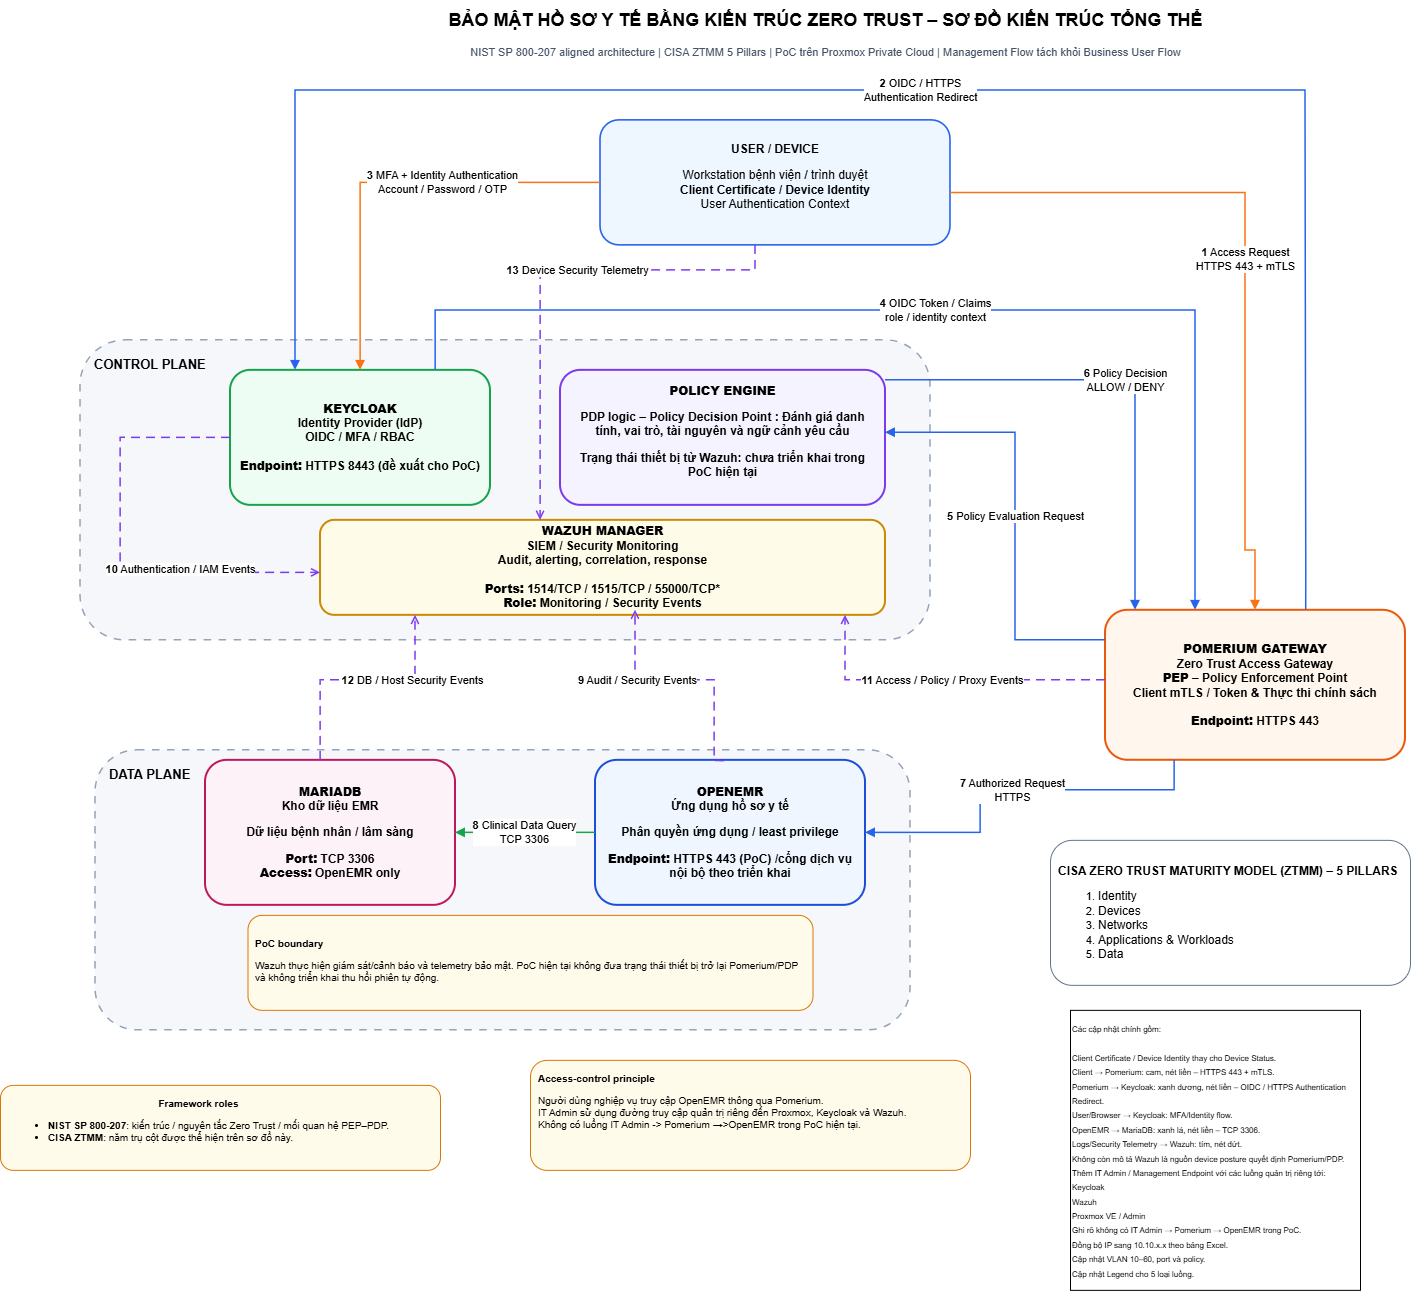
\includegraphics[width=0.95\textwidth]{image/zero_trust_overall_architecture_v2-Zero Trust Architecture.drawio.png}
    \caption{Sơ đồ kiến trúc tổng thể mô hình Zero Trust bảo mật Hồ sơ Y tế}
    \label{fig:overall_architecture}
\end{figure}

\subsubsection{Giải thích Chi tiết Sơ đồ Kiến trúc Tổng thể Mô hình Zero Trust (Hình 2.1)}

Sơ đồ kiến trúc tổng thể thể hiện mối quan hệ tương tác giữa 4 vùng thành phần chính: Vùng người dùng (Users/Devices), Vùng điều khiển truy cập (Access Control), Vùng ứng dụng \& dữ liệu (App \& Database), và Vùng giám sát an ninh (Security Monitoring).

Tạo tầng gác cổng uỷ quyền danh tính (Identity-Aware Proxy - Pomerium): Khi bác sĩ, kỹ thuật viên xét nghiệm hay nhân viên y tế truy cập từ thiết bị đầu cuối, luồng kết nối không đi trực tiếp vào máy chủ y tế mà bắt buộc phải trỏ tới Pomerium Access Gateway đóng vai trò Policy Enforcement Point (PEP). Pomerium kiểm tra chứng chỉ số cá thể (Client Certificate) được cài sẵn trên thiết bị thông qua giao thức mTLS để xác định thiết bị có thuộc danh sách được bệnh viện cấp phép hay không.

Tích hợp xác thực danh tính tập trung (Keycloak IdP): Khi kết nối mTLS hợp lệ, Pomerium chuyển hướng giao diện đăng nhập về Keycloak qua giao thức OIDC. Người dùng nhập tên tài khoản, mật khẩu và bắt buộc hoàn thành bước xác thực đa yếu tố (MFA) bằng việc nhập mã OTP từ ứng dụng Google Authenticator. Sau khi xác thực thành công, Keycloak trả về ID Token và Access Token chứa danh sách các vai trò (Roles) của người dùng.

Thực thi chính sách uỷ quyền ngữ cảnh (Policy Decision Point - PDP): Pomerium tiếp nhận Token từ Keycloak và đối chiếu với tập quy tắc Policy Route. Nếu vai trò của người dùng khớp với quyền hạn được phép truy cập tài nguyên y tế tương ứng, Pomerium mới khởi tạo kết nối uỷ quyền bảo mật (Authorized HTTPS) đưa lưu lượng vào ứng dụng OpenEMR. Các kết nối không đủ điều kiện xác thực hoặc sai vai trò sẽ bị Pomerium ra quyết định Deny và ngắt kết nối lập tức.

Bảo vệ vùng ứng dụng OpenEMR và cơ sở dữ liệu MariaDB: Máy chủ OpenEMR tiếp nhận luồng dữ liệu từ Pomerium và thực hiện phân quyền chi tiết RBAC ở tầng ứng dụng. Cơ sở dữ liệu MariaDB nằm ở phân đoạn mạng cô lập sâu nhất, chỉ chấp nhận kết nối duy nhất đến từ OpenEMR qua cổng TCP 3306. Dữ liệu trên MariaDB được mã hóa cấu trúc lưu trữ TDE (Encryption at Rest), đảm bảo an toàn tuyệt đối ngay cả khi tệp tin dữ liệu thô bị trích xuất ngoài ý muốn.

Tập trung giám sát an ninh và ghi nhận nhật ký (Wazuh SIEM/XDR): Tất cả các thành phần từ Pomerium, Keycloak, OpenEMR, MariaDB cho đến các máy ảo hạ tầng đều được cài đặt Wazuh Agent. Các nhật ký sự kiện (security events), nhật ký truy cập, cảnh báo đăng nhập thất bại và sự kiện thay đổi tệp tin cấu hình (FIM) đều được truyền liên tục về Wazuh Manager để phục vụ giám sát thời gian thực, phát cảnh báo và hỗ trợ truy vết an ninh.

\begingroup
\setlength\LTleft{0pt}
\setlength\LTright{0pt}
\begin{longtable}{| >{\raggedright\arraybackslash}p{3.2cm} | >{\raggedright\arraybackslash}p{5.5cm} | >{\raggedright\arraybackslash}p{5.5cm} |}
\caption{Bảng đối chiếu các công nghệ mã nguồn mở đáp ứng 5 trụ cột Zero Trust} \label{tab:cisa_mapping} \\
\hline
\textbf{Trụ cột / Năng lực} & \textbf{Tiêu chí bảo mật theo CISA} & \textbf{Công nghệ triển khai} \\ \hline
\endhead
\hline
\endfoot

Identity (Danh tính) & Xác thực người dùng, MFA, SSO, quản lý vai trò và phiên làm việc & Keycloak + Pomerium \\ \hline
Devices (Thiết bị) & Nhận diện thiết bị tin cậy, mTLS và theo dõi security posture & Client Certificate + mTLS + Wazuh Agent \\ \hline
Networks (Mạng) & Phân đoạn mạng logic, loại bỏ implicit trust, ngăn lateral movement & Proxmox VE Firewall + 6 VLANs + Pomerium Gateway \\ \hline
Applications \& Workloads & Bảo vệ ứng dụng OpenEMR, kiểm soát quyền truy cập theo context & Pomerium Policy + OpenEMR RBAC \\ \hline
Data (Dữ liệu) & Mã hóa đường truyền end-to-end và mã hóa dữ liệu lưu trữ tại ổ đĩa & TLS/HTTPS + MariaDB TDE Encryption \\ \hline
Visibility \& Analytics & Thu thập log tập trung, giám sát tính toàn vẹn và cảnh báo sự cố & Wazuh SIEM/XDR Manager + Agent \\ \hline
\end{longtable}
\endgroup

\subsection{Luồng Hoạt động Nghiệp vụ và Ma trận Phân quyền Chi tiết}

\subsubsection{Phân tích các Luồng Hoạt động Nghiệp vụ Cốt lõi (BF-01 đến BF-05)}

Dựa trên quy trình khám chữa bệnh và quản lý hồ sơ tại cơ sở y tế, hệ thống xác định năm luồng nghiệp vụ cốt lõi. Các luồng này thể hiện quá trình từ khi bệnh nhân được tiếp nhận, khám bệnh, thực hiện xét nghiệm cho đến khi hồ sơ bệnh án được lưu trữ, khai thác và phân công quản lý.

\textbf{Luồng nghiệp vụ BF-01 (Tiếp nhận bệnh nhân và tạo lượt khám):}
Nhân viên Lễ tân thực hiện tìm kiếm thông tin bệnh nhân trên hệ thống. Đối với bệnh nhân đã có hồ sơ, Lễ tân kiểm tra và cập nhật các thông tin hành chính cần thiết. Đối với bệnh nhân mới, Lễ tân nhập thông tin cá nhân để tạo hồ sơ bệnh nhân. Sau khi hoàn tất quá trình tiếp nhận, Lễ tân tạo lượt khám mới và ghi nhận các thông tin phục vụ việc khám bệnh. Phạm vi công việc của Lễ tân tập trung vào hoạt động tiếp nhận và quản lý thông tin hành chính của bệnh nhân, không bao gồm việc cập nhật các nội dung chuyên môn như chẩn đoán hoặc ghi chú lâm sàng.

\textbf{Luồng nghiệp vụ BF-02 (Khám bệnh, ghi chú lâm sàng và chẩn đoán):}
Sau khi bệnh nhân được tiếp nhận và tạo lượt khám, Bác sĩ tiến hành mở hồ sơ bệnh nhân để xem các thông tin cần thiết phục vụ quá trình khám. Bác sĩ thực hiện khám lâm sàng, ghi nhận triệu chứng, tiền sử liên quan, cập nhật ghi chú diễn biến và đưa ra chẩn đoán. Trong trường hợp cần thêm thông tin hỗ trợ chẩn đoán, Bác sĩ có thể tạo chỉ định xét nghiệm hoặc các dịch vụ cận lâm sàng phù hợp. Sau khi có đầy đủ thông tin, Bác sĩ tiếp tục cập nhật nội dung chuyên môn và hoàn thiện quá trình khám bệnh. Bác sĩ chỉ được cập nhật các nội dung chuyên môn đối với bệnh nhân và lượt khám thuộc phạm vi được phân công phụ trách; việc thay đổi thông tin chuyên môn của các lượt khám ngoài phạm vi phụ trách không được phép thực hiện. Trong trường hợp bệnh nhân cần tiếp tục điều trị nội trú, Bác sĩ có thể thực hiện chuyển bệnh nhân sang trạng thái nhập viện theo phạm vi nghiệp vụ của hệ thống. Quyền cập nhật hồ sơ nội trú sau đó chỉ áp dụng đối với Bác sĩ được phân công phụ trách bệnh nhân tương ứng.

\textbf{Luồng nghiệp vụ BF-03 (Chỉ định và xử lý kết quả xét nghiệm):}
Trong quá trình khám bệnh, khi cần thực hiện xét nghiệm, Bác sĩ tạo chỉ định xét nghiệm cho bệnh nhân. Kỹ thuật viên xét nghiệm tiếp nhận chỉ định, thực hiện xét nghiệm và cập nhật kết quả tương ứng. Trong thời gian xét nghiệm chưa hoàn tất, chỉ định có thể được điều chỉnh theo yêu cầu nghiệp vụ. Sau khi xét nghiệm đã hoàn thành và có kết quả, nội dung chỉ định liên quan không được thay đổi nhằm bảo đảm tính nhất quán giữa yêu cầu xét nghiệm và kết quả đã thực hiện. Sau khi kết quả xét nghiệm được xác nhận, Kỹ thuật viên xét nghiệm không được tiếp tục chỉnh sửa kết quả đó. Bác sĩ sử dụng kết quả đã xác nhận để hỗ trợ quá trình đánh giá tình trạng bệnh và hoàn thiện chẩn đoán.

\textbf{Luồng nghiệp vụ BF-04 (Khai thác hồ sơ bệnh án):}
Sau khi các thông tin khám bệnh được hình thành trong quá trình điều trị, hồ sơ bệnh án được lưu trữ để phục vụ nhu cầu quản lý và khai thác sau này. Nhân viên quản lý hồ sơ tiếp nhận các hồ sơ được phân công và thực hiện tra cứu thông tin bệnh nhân, lịch sử khám bệnh, tài liệu và các nội dung liên quan phục vụ nghiệp vụ quản lý hồ sơ. Nhân viên chỉ thực hiện khai thác những hồ sơ thuộc phạm vi công việc được giao và không tham gia chỉnh sửa các nội dung chuyên môn do Bác sĩ hoặc các bộ phận chuyên môn khác tạo ra.

\textbf{Luồng nghiệp vụ BF-05 (Phân công và chuyển giao hồ sơ bệnh án):}
Để quản lý phạm vi khai thác hồ sơ giữa các nhân viên, Medical Records Supervisor thực hiện phân công bệnh nhân hoặc hồ sơ bệnh án cho từng nhân viên quản lý hồ sơ. Sau khi được phân công, nhân viên quản lý hồ sơ chịu trách nhiệm khai thác các hồ sơ tương ứng phục vụ công việc. Khi có thay đổi về nhân sự hoặc yêu cầu nghiệp vụ, Medical Records Supervisor có thể chuyển giao hồ sơ từ nhân viên đang phụ trách sang một nhân viên khác. Sau khi quá trình chuyển giao hoàn tất, nhân viên mới tiếp nhận trách nhiệm quản lý hồ sơ theo phân công mới. Luồng nghiệp vụ này giúp xác định rõ trách nhiệm của từng nhân viên đối với từng nhóm hồ sơ bệnh án và hạn chế việc khai thác hồ sơ ngoài phạm vi công việc được giao.

\subsubsection{Ma trận Phân quyền Chi tiết (Granular Role-Permission Matrix)}

Ma trận phân quyền dưới đây quy định chi tiết các quyền thao tác gồm Đọc, Tạo, Sửa, Xóa và Xuất đối với từng loại tài nguyên trong hệ thống, dành cho 6 nhóm vai trò nghiệp vụ gồm Lễ tân, Bác sĩ, Kỹ thuật viên xét nghiệm, Nhân viên quản lý hồ sơ, Giám sát hồ sơ và Quản trị viên CNTT. Một số quyền chỉ được thực hiện khi thỏa mãn các điều kiện nghiệp vụ như bệnh nhân/lượt khám thuộc phạm vi phụ trách, hồ sơ đã được phân công thông qua Medical Records Assignment hoặc trạng thái xử lý của xét nghiệm.

\begin{landscape}

\begingroup
\small
\setlength{\tabcolsep}{3pt}
\renewcommand{\arraystretch}{1.15}
\setlength\LTleft{0pt}
\setlength\LTright{0pt}

\begin{longtable}{|
>{\raggedright\arraybackslash}p{2.3cm} |
>{\raggedright\arraybackslash}p{2.8cm} |
>{\centering\arraybackslash}p{1.1cm} |
>{\centering\arraybackslash}p{1.1cm} |
>{\centering\arraybackslash}p{1.1cm} |
>{\centering\arraybackslash}p{1.1cm} |
>{\centering\arraybackslash}p{1.2cm} |
>{\raggedright\arraybackslash}p{8.0cm} |
}

\caption{Ma trận phân quyền chi tiết Role-Permission Matrix trong hệ thống y tế}
\label{tab:rbac_granular_matrix} \\

\hline
\textbf{Vai trò} &
\textbf{Tài nguyên} &
\textbf{Đọc} &
\textbf{Tạo} &
\textbf{Sửa} &
\textbf{Xóa} &
\textbf{Xuất} &
\textbf{Điều kiện / Ghi chú nghiệp vụ} \\
\hline
\endfirsthead

\hline
\textbf{Vai trò} &
\textbf{Tài nguyên} &
\textbf{Đọc} &
\textbf{Tạo} &
\textbf{Sửa} &
\textbf{Xóa} &
\textbf{Xuất} &
\textbf{Điều kiện / Ghi chú nghiệp vụ} \\
\hline
\endhead

\hline
\endfoot

% ===================== LỄ TÂN =====================

Lễ tân &
Thông tin hành chính &
Có & Có & Có & Không & Không &
Chỉ xử lý các thông tin hành chính phục vụ quá trình tiếp nhận bệnh nhân. \\
\hline

Lễ tân &
Lượt khám &
Có & Có & Không & Không & Không &
Được tạo lượt khám mới khi tiếp nhận bệnh nhân; không được chỉnh sửa hoặc xóa dữ liệu chuyên môn của lượt khám. \\
\hline

Lễ tân &
Chẩn đoán &
Không & Không & Không & Không & Không &
Không thuộc phạm vi nghiệp vụ của Lễ tân. \\
\hline

Lễ tân &
Kết quả xét nghiệm &
Không & Không & Không & Không & Không &
Không thuộc phạm vi nghiệp vụ của Lễ tân. \\
\hline


% ===================== BÁC SĨ =====================

Bác sĩ &
Hồ sơ bệnh án &
Có & Không & Không & Không & Không &
Được đọc thông tin bệnh án phục vụ hoạt động khám và điều trị trong phạm vi được phép. \\
\hline

Bác sĩ &
Ghi chú lâm sàng &
Có & Có* & Có* & Không & Không &
Chỉ được tạo hoặc sửa đối với bệnh nhân và lượt khám thuộc phạm vi được phân công phụ trách. \\
\hline

Bác sĩ &
Chẩn đoán &
Có & Có* & Có* & Không & Không &
Chỉ được tạo hoặc sửa chẩn đoán đối với bệnh nhân và lượt khám thuộc phạm vi được phân công phụ trách. \\
\hline

Bác sĩ &
Chỉ định xét nghiệm &
Có & Có* & Có* & Không & Có* &
Được tạo chỉ định cho bệnh nhân thuộc phạm vi phụ trách. Chỉ được thay đổi nội dung chỉ định trước khi xét nghiệm được thực hiện và có kết quả. \\
\hline

Bác sĩ &
Kết quả xét nghiệm &
Có & Không & Không & Không & Không &
Được đọc kết quả xét nghiệm phục vụ chẩn đoán; không được tạo hoặc chỉnh sửa kết quả do bộ phận xét nghiệm phụ trách. \\
\hline


% ===================== KỸ THUẬT VIÊN XÉT NGHIỆM =====================

KTV Xét nghiệm &
Chỉ định xét nghiệm &
Có* & Không & Có* & Không & Không &
Được tiếp nhận chỉ định thuộc phạm vi xử lý và cập nhật trạng thái xử lý; không được thay đổi nội dung chỉ định do Bác sĩ tạo. \\
\hline

KTV Xét nghiệm &
Kết quả xét nghiệm &
Có* & Có* & Có* & Không & Có* &
Được nhập và cập nhật kết quả xét nghiệm thuộc phạm vi xử lý. Sau khi kết quả đã được xác nhận thì không được tiếp tục chỉnh sửa. \\
\hline

KTV Xét nghiệm &
Chẩn đoán &
Không & Không & Không & Không & Không &
Không thuộc phạm vi nghiệp vụ xét nghiệm. \\
\hline

KTV Xét nghiệm &
Ghi chú lâm sàng &
Không & Không & Không & Không & Không &
Không thuộc phạm vi nghiệp vụ xét nghiệm. \\
\hline


% ===================== NHÂN VIÊN QUẢN LÝ HỒ SƠ =====================

Quản lý hồ sơ &
Hồ sơ bệnh án &
Có* & Không & Không & Không & Có* &
Chỉ được đọc hoặc trích xuất khi bệnh nhân/hồ sơ đang được phân công cho chính nhân viên đó thông qua Medical Records Assignment. \\
\hline

Quản lý hồ sơ &
Tài liệu y tế &
Có* & Có* & Có* & Không & Có* &
Chỉ xử lý tài liệu thuộc bệnh nhân/hồ sơ đang được phân công; không được chỉnh sửa nội dung chuyên môn do Bác sĩ hoặc bộ phận chuyên môn tạo ra. \\
\hline

Quản lý hồ sơ &
Chẩn đoán &
Có* & Không & Không & Không & Không &
Chỉ được đọc khi bệnh nhân/hồ sơ đang được phân công; không được tạo, sửa hoặc xóa chẩn đoán. \\
\hline

Quản lý hồ sơ &
Ghi chú lâm sàng &
Có* & Không & Không & Không & Không &
Chỉ được đọc khi bệnh nhân/hồ sơ đang được phân công; không được tạo, sửa hoặc xóa ghi chú lâm sàng. \\
\hline

Quản lý hồ sơ &
Kết quả xét nghiệm &
Có* & Không & Không & Không & Không &
Chỉ được đọc khi bệnh nhân/hồ sơ đang được phân công; không được chỉnh sửa kết quả xét nghiệm. \\
\hline

Quản lý hồ sơ &
Thông tin phân công &
Có* & Không & Không & Không & Không &
Chỉ được xem thông tin phân công liên quan đến phạm vi của chính mình; không được tự assign hoặc reassign hồ sơ. \\
\hline


% ===================== GIÁM SÁT HỒ SƠ =====================

Giám sát hồ sơ &
Thông tin phân công &
Có & Có & Có & Không & Không &
Được thực hiện assign và reassign bệnh nhân/hồ sơ cho Nhân viên quản lý hồ sơ. \\
\hline

Giám sát hồ sơ &
Thông tin hành chính &
Có* & Không & Không & Không & Không &
Chỉ được xem các thông tin tối thiểu cần thiết để xác định đúng bệnh nhân khi thực hiện phân công hồ sơ. \\
\hline

Giám sát hồ sơ &
Dữ liệu chuyên môn &
Không & Không & Không & Không & Không &
Quyền quản lý việc phân công hồ sơ không đồng nghĩa với quyền truy cập hoặc chỉnh sửa nội dung chuyên môn của bệnh án. \\
\hline


% ===================== IT ADMIN =====================

IT Admin &
Tài khoản / Role &
Có & Có & Có & Không & Không &
Quản lý tài khoản và vai trò người dùng; khi tài khoản không còn được sử dụng thì thực hiện vô hiệu hóa thay vì xóa. \\
\hline

IT Admin &
Bảo mật / Log &
Có & Không & Có & Không & Không &
Thực hiện các thao tác quản trị kỹ thuật và cấu hình bảo mật trong phạm vi được cấp. \\
\hline

IT Admin &
Hồ sơ bệnh án &
Không & Không & Không & Không & Không &
Quyền quản trị hệ thống không mặc định đồng nghĩa với quyền đọc hoặc chỉnh sửa nội dung hồ sơ bệnh án. \\
\hline

\end{longtable}

\endgroup

\end{landscape}

\noindent\textit{Ghi chú quy ước trong bảng:}
\begin{itemize}
    \item \textbf{Có}: Quyền được cấp theo vai trò.
    \item \textbf{Có*}: Quyền được cấp có điều kiện; phải thỏa mãn ràng buộc tại cột ``Điều kiện / Ghi chú nghiệp vụ''.
    \item \textbf{Không}: Quyền không được cấp.
\end{itemize}

\subsection{Chi tiết các Công nghệ Triển khai và Lý do Lựa chọn}

\subsubsection{Hệ thống Quản lý Danh tính tập trung Keycloak}

\textbf{Tại sao lựa chọn sử dụng Keycloak:} Keycloak là giải pháp Quản lý Danh tính và Truy cập (IAM/IdP) mã nguồn mở hàng đầu hiện nay, hỗ trợ đầy đủ các chuẩn xác thực hiện đại như OIDC, OAuth 2.0 và SAML 2.0, có khả năng mở rộng cao và tích hợp dễ dàng với các dịch vụ uỷ quyền.

\textbf{Mục đích sử dụng cụ thể:} Keycloak được dùng làm máy chủ Identity Provider (IdP) trung tâm cho toàn bộ hệ thống y tế. Keycloak đảm nhận nhiệm vụ lưu trữ tài khoản người dùng, quản lý vai trò (Role-Based Access Control - RBAC), bắt buộc người dùng thực hiện xác thực đa yếu tố (MFA qua Google Authenticator/OTP) và cung cấp cơ chế Đăng nhập một lần (SSO) cho toàn bộ nhân viên y tế.

\subsubsection{Cổng Uỷ quyền Nhận biết Danh tính Pomerium (Identity-Aware Proxy)}

\textbf{Tại sao lựa chọn sử dụng Pomerium:} Pomerium là giải pháp Access Proxy độc lập hoạt động theo kiến trúc Zero Trust (ZTNA), cho phép kiểm tra quyền truy cập ở cấp độ HTTP/HTTPS request dựa trên danh tính người dùng được trả về từ IdP mà không cần cài đặt VPN client phức tạp.

\textbf{Mục đích sử dụng cụ thể:} Pomerium đóng vai trò là trạm gác Policy Enforcement Point (PEP) đứng trước hệ thống y tế. Mọi luồng truy cập của bác sĩ, kỹ thuật viên xét nghiệm, nhân viên y tế hay quản trị viên từ bên ngoài hoặc mạng nội bộ bắt buộc phải đi qua Pomerium. Pomerium sẽ liên kết với Keycloak qua OIDC để xác thực danh tính, kiểm tra chứng chỉ thiết bị (mTLS) và áp dụng các chính sách Allow/Deny định tuyến truy cập vào ứng dụng.

\subsubsection{Hệ thống Hồ sơ Y tế Điện tử OpenEMR}

\textbf{Tại sao lựa chọn sử dụng OpenEMR:}  
OpenEMR là phần mềm quản lý phòng khám và hồ sơ sức khỏe điện tử mã nguồn mở, cung cấp nhiều chức năng nghiệp vụ y tế như quản lý thông tin bệnh nhân, lượt khám, ghi chú lâm sàng, chẩn đoán, chỉ định xét nghiệm và kết quả xét nghiệm. OpenEMR đồng thời hỗ trợ cơ chế phân quyền theo vai trò và có khả năng tùy biến, phù hợp để xây dựng môi trường thử nghiệm cho các yêu cầu kiểm soát truy cập trong kiến trúc Zero Trust. OpenEMR hiện cũng có phiên bản được chứng nhận theo chương trình ONC Certified Health IT. 

\textbf{Mục đích sử dụng cụ thể:}  
OpenEMR được sử dụng làm hệ thống quản lý hồ sơ y tế trung tâm trong mô hình thử nghiệm. Nhóm xây dựng và kiểm thử các vai trò gồm Lễ tân, Bác sĩ, Kỹ thuật viên xét nghiệm, Nhân viên quản lý hồ sơ, Giám sát hồ sơ và Quản trị viên CNTT; đồng thời áp dụng ACL/GACL để kiểm soát chức năng của từng vai trò. Đối với nghiệp vụ quản lý hồ sơ, cơ chế Medical Records Assignment được bổ sung để giới hạn Nhân viên quản lý hồ sơ chỉ được truy cập những bệnh nhân đã được phân công, trong khi Giám sát hồ sơ thực hiện việc phân công hoặc chuyển giao hồ sơ.

\subsubsection{Hệ quản trị Cơ sở Dữ liệu MariaDB và Cơ chế Mã hóa Dữ liệu Lưu trữ}

\textbf{Tại sao lựa chọn sử dụng MariaDB TDE:} MariaDB là hệ quản trị cơ sở dữ liệu quan hệ mạnh mẽ, tương thích hoàn toàn với OpenEMR và tích hợp sẵn tính năng mã hóa dữ liệu trong suốt Transparent Data Encryption (TDE) thông qua plugin \url{file_key_management}.

\textbf{Mục đích sử dụng cụ thể:} MariaDB đảm nhận vai trò lưu trữ toàn bộ dữ liệu cơ sở của OpenEMR. Dự án kích hoạt cơ chế Data-at-Rest Encryption trên MariaDB để mã hóa toàn bộ các tệp tin lưu trữ dữ liệu (.ibd) trên ổ đĩa vật lý. Điều này đảm bảo nếu kẻ tấn công lấy cắp được ổ cứng vật lý hoặc tệp tin dữ liệu thô cũng không thể đọc được thông tin bệnh nhân nếu không có khóa master key.

\subsubsection{Hệ thống Cấp phát Chứng chỉ Easy-RSA và Xác thực Thiết bị mTLS}

\textbf{Tại sao lựa chọn sử dụng Easy-RSA và mTLS:} Easy-RSA là công cụ quản lý hạ tầng khóa công khai (PKI) nhỏ gọn, đáng tin cậy. Giao thức Mutual TLS (mTLS) cho phép xác thực hai chiều giữa client và server thông qua chứng chỉ số X.509 mà không thể bị giả mạo bởi địa chỉ IP hay MAC.

\textbf{Mục đích sử dụng cụ thể:} Easy-RSA được sử dụng để khởi tạo một Certificate Authority (CA) nội bộ cho hệ thống. CA này phát hành các chứng chỉ số cá thể (Client Certificates) cài đặt lên các thiết bị đầu cuối được bệnh viện cấp phép. Pomerium sẽ cấu hình mTLS bắt buộc; các thiết bị truy cập nếu không sở hữu chứng chỉ số hợp lệ do CA nội bộ cấp sẽ bị từ chối truy cập ngay tại tầng giao vận TLS.

\subsubsection{Hệ thống Giám sát An ninh Điểm cuối Wazuh SIEM/XDR}

\textbf{Tại sao lựa chọn sử dụng Wazuh:} Wazuh là nền tảng giám sát an ninh mạng và bảo vệ điểm cuối mã nguồn mở mạnh mẽ, cung cấp khả năng phát hiện đe dọa, giám sát tính toàn vẹn của tệp tin (FIM) và thu thập log tập trung theo thời gian thực.

\textbf{Mục đích sử dụng cụ thể:} Wazuh Agent được cài đặt lên tất cả các máy chủ ảo (VM) và thiết bị người dùng, truyền dữ liệu về Wazuh Manager tập trung. Wazuh đảm nhận nhiệm vụ giám sát sự thay đổi của các tệp tin cấu hình hệ thống, phát hiện các hành vi vô hiệu hóa tường lửa, ghi nhận các nỗ lực đăng nhập thất bại và phát cảnh báo tức thì cho quản trị viên an ninh.

\subsubsection{Nền tảng Ảo hóa Proxmox VE và Cơ chế Phân đoạn Mạng Logic}

\textbf{Tại sao lựa chọn sử dụng Proxmox VE:} Proxmox Virtual Environment (VE) là nền tảng ảo hóa doanh nghiệp mã nguồn mở tích hợp sẵn công nghệ Linux Bridge VLAN-aware và Proxmox Firewall, cho phép quản lý linh hoạt hạ tầng ảo và phân đoạn mạng an toàn.

\textbf{Mục đích sử dụng cụ thể:} Proxmox VE được sử dụng làm hạ tầng Hypervisor lưu trữ toàn bộ các máy chủ ảo của dự án. Proxmox VE cấu hình cầu nối VLAN-aware bridge (`vmbr1`) chia hệ thống thành 6 phân đoạn VLAN logic (Client, DMZ, Security, App, DB, Management). Proxmox Firewall được áp dụng để chặn toàn bộ kết nối trực tiếp từ người dùng vào máy chủ App và DB, bắt buộc mọi kết nối phải đi qua cổng Pomerium Proxy.

    \newpage
    \clearpage

    \section{THỰC NGHIỆM}

\subsection{Thiết kế Hợp đồng Cấu hình (Config Contract) và Sơ đồ Mạng PoC}

Để đảm bảo tính nhất quán và đồng bộ giữa các thành phần triển khai, dự án đã xây dựng một Hợp đồng Cấu hình chuẩn hóa làm nguồn sự thật duy nhất (Single Source of Truth) lưu giữ dưới tệp tin \texttt{CONFIG\_CONTRACT.yaml}. Hợp đồng này quy định chi tiết địa chỉ IP, cổng dịch vụ, phân đoạn VLAN và phiên bản phần mềm cho toàn bộ 5 máy chủ ảo trong hệ thống.

Mạng nội bộ được quy hoạch chi tiết trên dải IP \texttt{10.10.x.x} và phân chia thành 6 vùng mạng ảo (VLAN) logic độc lập nhằm triệt tiêu niềm tin ngầm định theo vị trí kết nối.

\begin{table}[H]
\centering
\caption{Bảng quy hoạch phân đoạn VLAN và địa chỉ IP hệ thống}
\label{tab:vlan_mapping}
\begin{tabular}{| c | p{3.2cm} | p{3.2cm} | p{2.8cm} | p{2.5cm} |}
\hline
\textbf{VLAN ID} & \textbf{Phân đoạn / Zone} & \textbf{Subnet IP} & \textbf{Gateway IP} & \textbf{Mục đích / Ghi chú} \\ \hline
10 & Client Zone & 10.10.10.0/24 & 10.10.10.1 & Thiết bị người dùng (DHCP) \\ \hline
20 & DMZ Zone & 10.10.20.0/24 & 10.10.20.1 & Pomerium Gateway (10.10.20.10) \\ \hline
30 & Security Zone & 10.10.30.0/24 & 10.10.30.1 & Keycloak IAM \& Wazuh Manager \\ \hline
40 & App Zone & 10.10.40.0/24 & 10.10.40.1 & Máy chủ ứng dụng OpenEMR \\ \hline
50 & DB Zone & 10.10.50.0/24 & 10.10.50.1 & Cơ sở dữ liệu MariaDB TDE \\ \hline
60 & Management Zone & 10.10.60.0/24 & 10.10.60.1 & Quản trị Proxmox VE (10.10.60.10) \\ \hline
\end{tabular}
\end{table}

\begin{figure}[H]
    \centering
    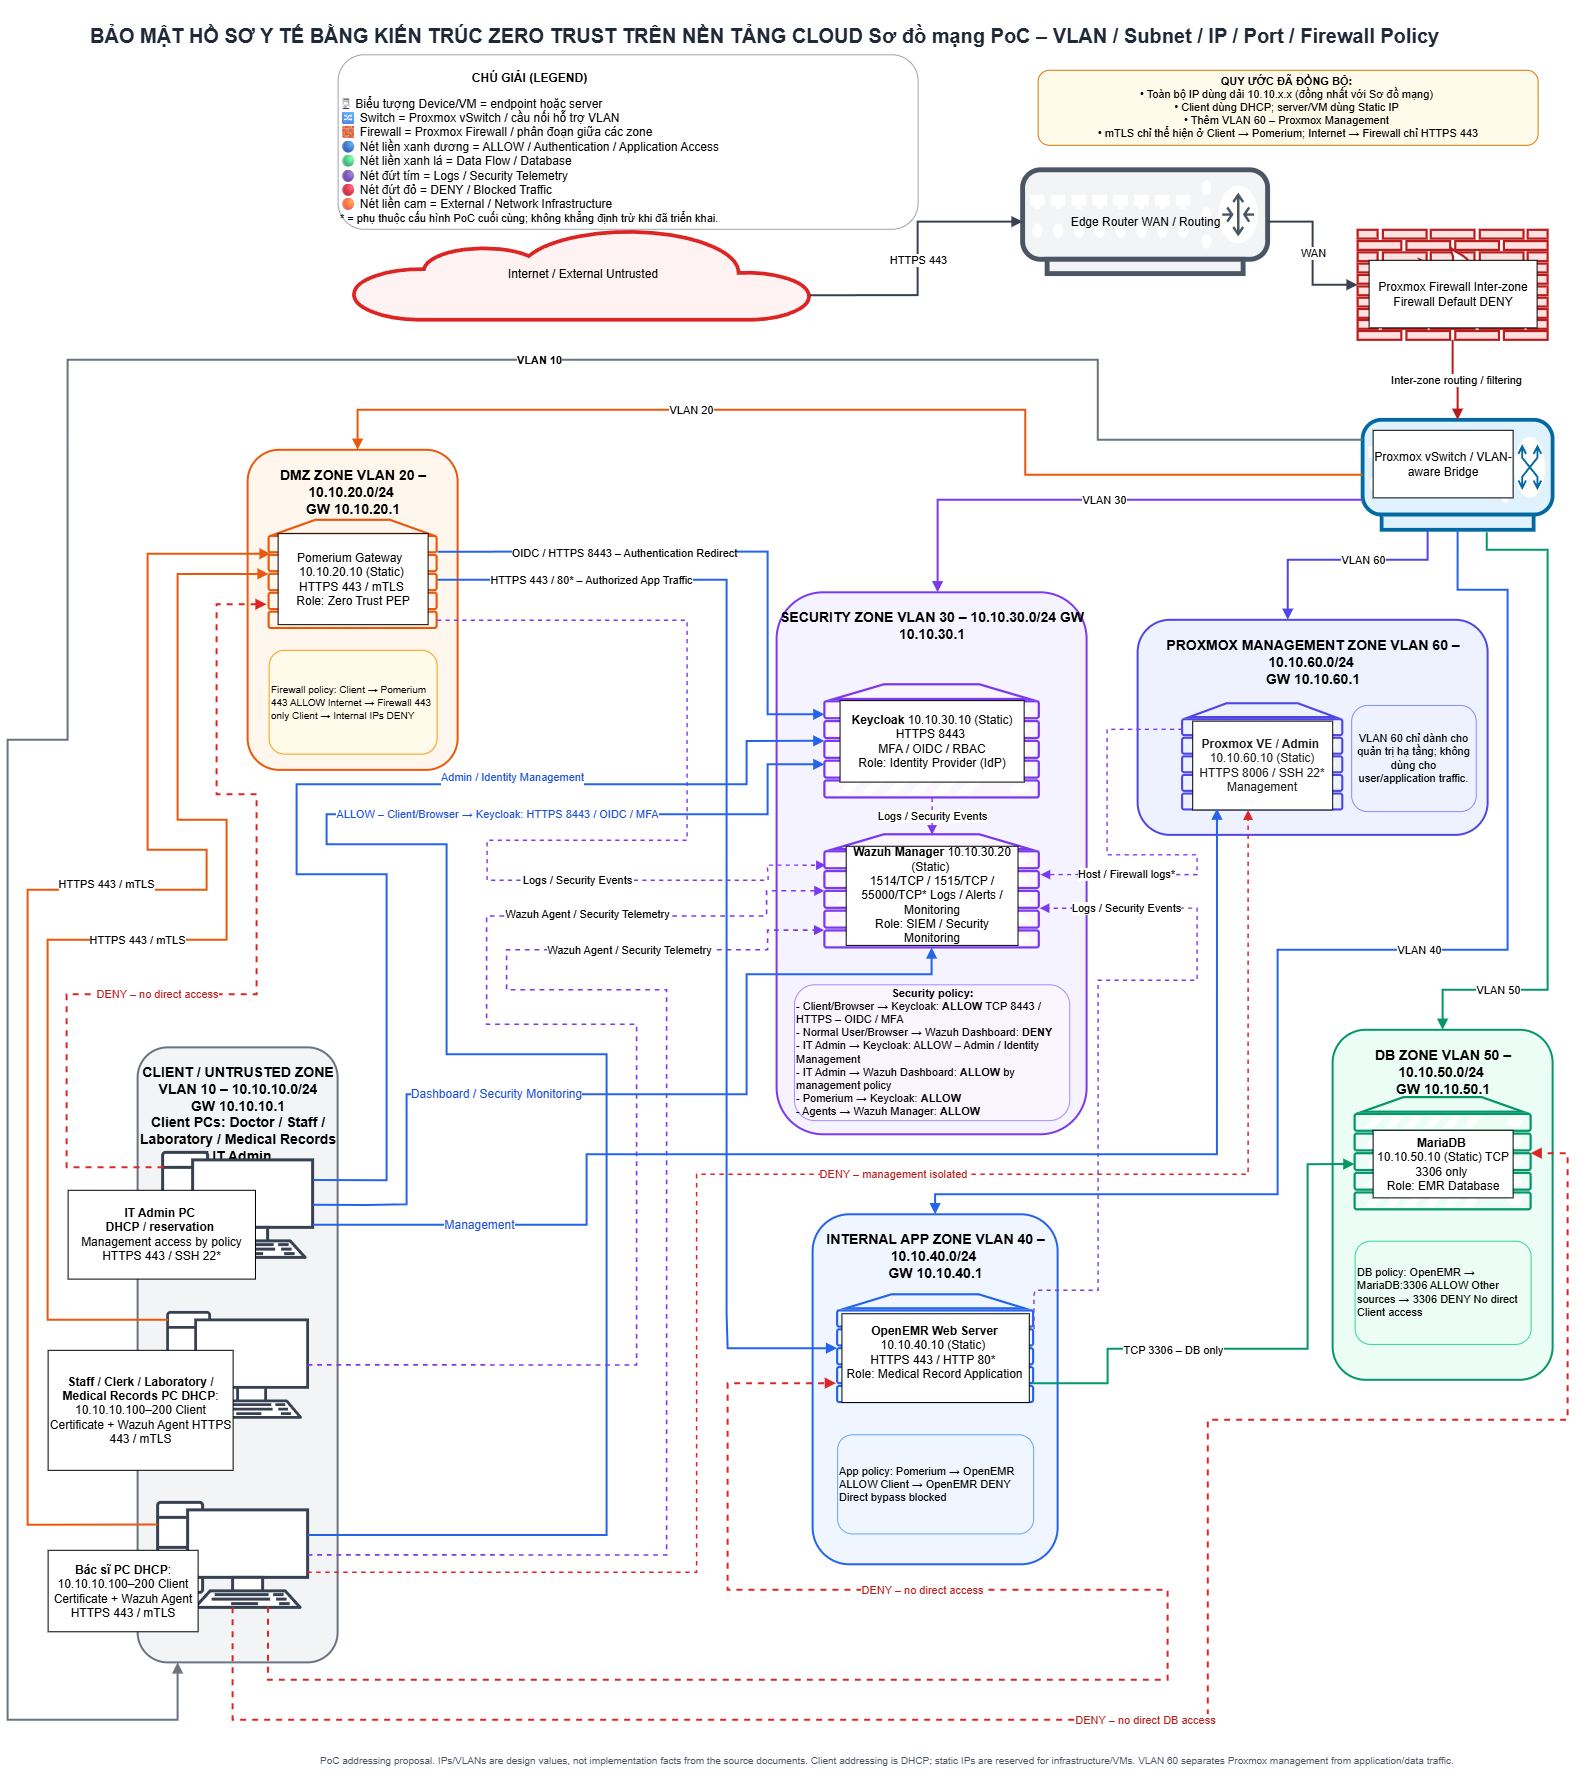
\includegraphics[width=0.95\textwidth]{image/zero_trust_medical_network_diagram_v3.drawio.png}
    \caption{Sơ đồ thiết kế phân đoạn mạng PoC Zero Trust bảo mật Hồ sơ Y tế Điện tử}
    \label{fig:network_diagram}
\end{figure}

\subsubsection{Giải thích Chi tiết Sơ đồ Thiết kế Mạng PoC (Hình 3.1)}

Sơ đồ thiết kế mạng PoC mô tả chi tiết hạ tầng mạng ảo hóa phân đoạn thành 6 vùng VLAN riêng biệt, quy định chặt chẽ các luồng dữ liệu được phép (ALLOW), luồng bị cấm (DENY) và luồng giám sát an ninh (Security Telemetry).

Phân đoạn 6 vùng VLAN cô lập: VLAN10 Client Zone (\texttt{10.10.10.0/\allowbreak 24}) chứa các thiết bị của người dùng (bác sĩ, kỹ thuật viên xét nghiệm, nhân viên y tế) kết nối; VLAN20 DMZ Zone (\texttt{10.10.20.0/\allowbreak 24}) đặt Pomerium Gateway tại IP \texttt{10.10.20.10}; VLAN30 Security Zone (\texttt{10.10.30.0/\allowbreak 24}) chứa Keycloak IAM (\texttt{10.10.30.10}) và Wazuh Manager (\texttt{10.10.30.20}); VLAN40 App Zone (\texttt{10.10.40.0/\allowbreak 24}) chứa máy chủ OpenEMR (\texttt{10.10.40.10}); VLAN50 DB Zone (\texttt{10.10.50.0/\allowbreak 24}) chứa MariaDB (\texttt{10.10.50.10}); và VLAN60 Management Zone (\texttt{10.10.60.0/\allowbreak 24}) dành riêng cho quản trị hypervisor Proxmox VE (\texttt{10.10.60.10}).

Phân tích các luồng mạng được cấp phép (ALLOW Traffic Paths): Người dùng truy cập từ VLAN10 gửi yêu cầu HTTPS 443 tới Pomerium Gateway tại VLAN20 kèm chứng chỉ mTLS. Pomerium gửi yêu cầu xác thực sang Keycloak tại VLAN30 qua OIDC HTTPS 8443. Khi người dùng hoàn thành xác thực và MFA, Pomerium chuyển tiếp lưu lượng được uỷ quyền (Authorized Traffic) sang OpenEMR tại VLAN40. Máy chủ OpenEMR kết nối truy vấn dữ liệu tới MariaDB tại VLAN50 duy nhất qua cổng TCP 3306.

Phân tích các luồng kết nối bị từ chối (DENY Traffic Paths - Nét đứt màu đỏ): Để triệt tiêu khả năng truy cập bypass cổng uỷ quyền và ngăn chặn di chuyển ngang (Lateral Movement), Tường lửa Proxmox Firewall thiết lập các quy tắc chặn tuyệt đối: Client không được phép truy cập trực tiếp vào OpenEMR (\texttt{Client -> OpenEMR: DENY}); Client tuyệt đối không có luồng kết nối tới MariaDB (\texttt{Client -> MariaDB: DENY}); và vùng Management cô lập hoàn toàn với dữ liệu ứng dụng.

Phân tích các luồng giám sát an ninh (Security Telemetry - Nét đứt màu tím): Tất cả các nút thành phần bao gồm thiết bị người dùng, Pomerium Gateway, Keycloak IAM, OpenEMR Web Server và Proxmox Hypervisor đều liên tục đẩy nhật ký sự kiện an ninh và telemetry về máy chủ trung tâm Wazuh Manager tại VLAN30 để theo dõi và phát cảnh báo thời gian thực.

\subsection{Triển khai Hạ tầng Ảo hóa Proxmox VE và 5 Máy chủ Ảo Skeleton}

Hệ thống ảo hóa được triển khai trên máy chủ Proxmox VE phiên bản 9.2-1 với hostname \texttt{pve01}. Cầu nối ảo mạng nội bộ \texttt{vmbr1} được cấu hình hỗ trợ \texttt{bridge-vlan-aware yes} với danh sách các VLAN ID từ 10 đến 60.

Năm máy chủ ảo Linux Debian skeleton đã được khởi tạo thành công trên Proxmox VE với cấu hình card mạng kép: một card kết nối mạng Internet tạm thời \texttt{vmbr0} để cập nhật gói tin và một card kết nối mạng nội bộ Zero Trust \texttt{vmbr1} được gán thẻ VLAN tương ứng.

\begin{table}[H]
\centering
\caption{Danh sách thông số chi tiết 5 máy chủ ảo Skeleton trên Proxmox VE}
\label{tab:vm_skeletons}
\begin{tabular}{| c | p{2.8cm} | c | c | c | c | p{3.2cm} |}
\hline
\textbf{VMID} & \textbf{Tên máy chủ ảo} & \textbf{VLAN} & \textbf{vCPU} & \textbf{RAM} & \textbf{Disk} & \textbf{Giao diện mạng nội bộ (net1)} \\ \hline
100 & emr-app01 & 40 & 2 & 2048MB & 32GB & vmbr1, tag=40 (VLAN40 App) \\ \hline
101 & zt-pomerium01 & 20 & 2 & 2048MB & 32GB & vmbr1, tag=20 (VLAN20 DMZ) \\ \hline
102 & zt-keycloak01 & 30 & 2 & 2048MB & 32GB & vmbr1, tag=30 (VLAN30 Security) \\ \hline
103 & zt-wazuh01 & 30 & 2 & 2048MB & 32GB & vmbr1, tag=30 (VLAN30 Security) \\ \hline
104 & emr-db01 & 50 & 2 & 2048MB & 32GB & vmbr1, tag=50 (VLAN50 DB) \\ \hline
\end{tabular}
\end{table}

\subsection{Cấu hình Hệ thống IAM Keycloak và Ma trận Phân quyền RBAC}

Máy chủ Keycloak được cài đặt trên VM102 và cấu hình Realm dành riêng cho hệ thống y tế mang tên \texttt{Hospital-Realm}.

Keycloak tiến hành định nghĩa các vai trò (Roles) cốt lõi phản ánh đúng cơ cấu tổ chức và ma trận phân quyền phòng khám bao gồm Doctor (Bác sĩ), Receptionist (Lễ tân), Lab (Kỹ thuật viên xét nghiệm), Records (Nhân viên quản lý hồ sơ), Medical Records Supervisor (Giám sát hồ sơ) và IT Admin (Quản trị viên CNTT).

Các tài khoản người dùng được tạo lập thử nghiệm và gán đúng vai trò tương ứng. Đồng thời, chính sách bảo mật bắt buộc cấu hình xác thực đa yếu tố (MFA) được kích hoạt. Khi đăng nhập lần đầu, người dùng bắt buộc phải sử dụng ứng dụng Google Authenticator trên điện thoại thông minh để quét mã QR và nhập mã OTP 6 chữ số.

\subsection{Cấu hình Cổng Uỷ quyền Pomerium và Tích hợp OIDC / mTLS}

Máy chủ Pomerium Gateway được cài đặt trên VM101, đóng vai trò trạm gác duy nhất tiếp nhận các kết nối HTTPS từ bên ngoài.

Pomerium được cấu hình tích hợp với Keycloak thông qua giao thức OpenID Connect (OIDC). Tệp tin cấu hình \url{config.yaml} của Pomerium khai báo \url{identity_provider_url} trỏ về Keycloak Realm và xác thực client secret.

Pomerium thiết lập các quy tắc phân luồng chính sách (Policy Routes): các yêu cầu định tuyến tới địa chỉ \url{https://emr.hospital.local} chỉ được cấp phép (Allow) nếu người dùng đã xác thực thành công qua Keycloak và sở hữu vai trò hợp lệ.

Để đảm bảo nhận diện thiết bị tin cậy, Pomerium được tích hợp chứng chỉ CA nội bộ được khởi tạo từ Easy-RSA. Pomerium bật tính năng xác thực hai chiều \url{downstream_client_ca}; các thiết bị người dùng nếu không được cài đặt chứng chỉ cá thể (.pfx/.crt) do CA nội bộ cấp sẽ bị từ chối kết nối ngay tại tầng giao vận TLS.

\subsection{Triển khai OpenEMR, MariaDB TDE và Giám sát Wazuh}

Ứng dụng OpenEMR được triển khai trên VM100 và được sử dụng làm hệ thống quản lý hồ sơ y tế trung tâm trong mô hình PoC. Theo kiến trúc, OpenEMR sẽ kết nối tới cơ sở dữ liệu MariaDB trên VM104 thông qua mạng nội bộ giữa VLAN40 và VLAN50 

Trên OpenEMR, nhóm xây dựng các vai trò nghiệp vụ gồm Lễ tân (\texttt{receptionist}), Bác sĩ (\texttt{doctor}), Kỹ thuật viên xét nghiệm (\texttt{lab}), Nhân viên quản lý hồ sơ (\texttt{records}), Giám sát hồ sơ (\texttt{medicalrecordssupervisor}) và Quản trị viên CNTT (\texttt{itadmin}). Tài khoản \texttt{admin} được sử dụng cho mục đích cấu hình và quản trị hệ thống ở mức cao nhất, không được xem là một actor nghiệp vụ trong ma trận phân quyền.

Cơ chế ACL/GACL của OpenEMR được sử dụng để giới hạn các chức năng mà từng vai trò được phép thực hiện theo ma trận phân quyền đã xác định ở Chương 2. Lễ tân được giới hạn ở các chức năng tiếp nhận và thông tin hành chính; Bác sĩ thực hiện các nghiệp vụ khám bệnh, ghi chú lâm sàng, chẩn đoán và chỉ định xét nghiệm; Kỹ thuật viên xét nghiệm xử lý chỉ định và kết quả xét nghiệm; Nhân viên quản lý hồ sơ khai thác hồ sơ trong phạm vi được phân công; Quản trị viên CNTT thực hiện các chức năng quản trị kỹ thuật nhưng không mặc định có quyền truy cập nội dung hồ sơ bệnh án.

Đối với vai trò Bác sĩ, quyền cập nhật dữ liệu chuyên môn được giới hạn theo bệnh nhân và lượt khám thuộc phạm vi phụ trách. Bác sĩ được phép tạo hoặc cập nhật ghi chú lâm sàng, chẩn đoán và chỉ định xét nghiệm đối với lượt khám thuộc phạm vi được phân công. Khi xét nghiệm đã được thực hiện và có kết quả, nội dung chỉ định liên quan không được tiếp tục thay đổi nhằm bảo đảm tính nhất quán giữa chỉ định và kết quả xét nghiệm.

Đối với vai trò Kỹ thuật viên xét nghiệm, người dùng được phép tiếp nhận chỉ định, cập nhật trạng thái xử lý và nhập kết quả xét nghiệm trong phạm vi nghiệp vụ được giao. Kỹ thuật viên xét nghiệm không được chỉnh sửa chẩn đoán hoặc ghi chú lâm sàng của Bác sĩ. Sau khi kết quả xét nghiệm đã được xác nhận, kết quả không được tiếp tục chỉnh sửa.

Bên cạnh phân quyền theo vai trò, nhóm bổ sung cơ chế \textit{Medical Records Assignment} nhằm giới hạn phạm vi bệnh nhân mà Nhân viên quản lý hồ sơ được phép truy cập. Vai trò \texttt{medicalrecordssupervisor} chịu trách nhiệm thực hiện assign hoặc reassign bệnh nhân cho người dùng thuộc vai trò \texttt{records}. Khi Nhân viên quản lý hồ sơ truy cập một bệnh nhân, hệ thống kiểm tra thông tin phân công trước khi cho phép khai thác các khu vực hồ sơ được bảo vệ. Nhân viên quản lý hồ sơ không được tự assign hoặc reassign hồ sơ cho chính mình, trong khi quyền quản lý assignment của Medical Records Supervisor không đồng nghĩa với quyền truy cập hoặc chỉnh sửa dữ liệu chuyên môn của bệnh án.

Trên VM104, cơ sở dữ liệu MariaDB được cấu hình kích hoạt tính năng mã hóa dữ liệu lưu trữ Transparent Data Encryption (TDE) thông qua plugin \url{file_key_management}. Tệp tin chìa khóa mã hóa được lưu trữ bảo mật và cấp quyền truy cập hạn chế cho dịch vụ mysql.

Dịch vụ giám sát Wazuh Manager được thiết lập trên VM103. Wazuh Agent được cài đặt lên tất cả 5 máy chủ ảo và cấu hình kết nối về Manager qua cổng 1514/1515. Wazuh kích hoạt mô-đun File Integrity Monitoring (FIM) theo dõi trực tiếp các tệp tin cấu hình nhạy cảm như \url{/etc/pomerium/config.yaml}, \url{/etc/mysql/mariadb.conf.d/} và phát cảnh báo tức thì khi có sự thay đổi trái phép.

Tường lửa Proxmox Firewall được thiết lập quy tắc chặn toàn bộ (Drop All) các kết nối mạng trực tiếp từ phân đoạn VLAN10 (Client) tới VLAN40 (App) và VLAN50 (DB), buộc tất cả lưu lượng bắt buộc phải đi qua đại diện uỷ quyền Pomerium Gateway tại VLAN20.

    \newpage
    \clearpage

    \section{KẾT QUẢ VÀ ĐÁNH GIÁ}

\subsection{Kết quả Thực nghiệm Bộ Kịch bản Kiểm thử}

Bộ kiểm thử của hệ thống được xây dựng gồm 22 kịch bản từ TC-01 đến TC-22, bao phủ các nhóm kiểm soát chính gồm xác thực danh tính và MFA, xác thực thiết bị, kiểm soát truy cập qua Pomerium, phân đoạn mạng, phân quyền RBAC ở tầng OpenEMR, kiểm soát truy cập theo ngữ cảnh, Medical Records Assignment, giám sát an ninh và bảo vệ dữ liệu.

Các kịch bản kiểm thử được xây dựng theo cả hai hướng Allow và Deny nhằm đánh giá không chỉ các luồng truy cập hợp lệ mà còn các trường hợp người dùng có vai trò hợp lệ nhưng không thỏa mãn điều kiện về phạm vi bệnh nhân, lượt khám, phân công hồ sơ hoặc trạng thái xử lý. 

\begingroup
\setlength\LTleft{0pt}
\setlength\LTright{0pt}

\begin{longtable}{|
>{\centering\arraybackslash}p{1.1cm} |
>{\raggedright\arraybackslash}p{4.8cm} |
>{\raggedright\arraybackslash}p{4.8cm} |
>{\raggedright\arraybackslash}p{3.5cm} |
}

\caption{Bảng tổng hợp 22 kịch bản kiểm thử hệ thống Zero Trust}
\label{tab:testcases_summary} \\

\hline
\textbf{Mã TC} &
\textbf{Kịch bản kiểm thử} &
\textbf{Kết quả mong đợi} &
\textbf{Tiêu chí Zero Trust} \\
\hline
\endfirsthead

\hline
\textbf{Mã TC} &
\textbf{Kịch bản kiểm thử} &
\textbf{Kết quả mong đợi} &
\textbf{Tiêu chí Zero Trust} \\
\hline
\endhead

\hline
\endfoot

TC-01 &
Người dùng hợp lệ truy cập OpenEMR qua luồng Zero Trust đầy đủ với tài khoản, OTP và Client Certificate hợp lệ. &
Certificate, tài khoản, OTP và phiên đều hợp lệ; Pomerium cho phép định tuyến tới OpenEMR. &
Identity / MFA / Device Trust / Gateway Enforcement \\
\hline

TC-02 &
Người dùng đăng nhập bằng tài khoản hoặc mật khẩu không hợp lệ. &
Không tạo phiên xác thực; người dùng không truy cập được OpenEMR và sự kiện đăng nhập thất bại được ghi nhận. &
Explicit Verification / Identity \\
\hline

TC-03 &
Người dùng nhập thiếu hoặc sai mã OTP trong quá trình xác thực đa yếu tố. &
Quá trình xác thực không hoàn tất; không cấp phiên truy cập OpenEMR. &
MFA / Explicit Verification \\
\hline

TC-04 &
Thiết bị không có Client Certificate hoặc sử dụng chứng chỉ không hợp lệ truy cập hệ thống. &
Yêu cầu bị chặn tại lớp truy cập trước khi tới OpenEMR. &
Device Trust / mTLS \\
\hline

TC-05 &
Người dùng gửi yêu cầu tới OpenEMR khi không có phiên xác thực hợp lệ. &
Pomerium từ chối yêu cầu hoặc yêu cầu xác thực lại; request không được chuyển tới OpenEMR. &
Identity / Session Verification \\
\hline

TC-06 &
Client cố gắng truy cập trực tiếp OpenEMR để bypass Pomerium Gateway. &
Kết nối trực tiếp bị Proxmox Firewall chặn. &
Gateway Enforcement / Network Segmentation \\
\hline

TC-07 &
Lễ tân quản lý thông tin hành chính bệnh nhân và tạo lượt khám mới. &
Cho phép đọc, tạo, cập nhật thông tin hành chính và tạo lượt khám theo đúng quyền của vai trò. &
RBAC / Least Privilege \\
\hline

TC-08 &
Lễ tân cố gắng thao tác trên Chẩn đoán hoặc Kết quả xét nghiệm. &
Các thao tác nằm ngoài phạm vi quyền của Lễ tân bị từ chối. &
RBAC / Least Privilege \\
\hline

TC-09 &
Bác sĩ đọc hồ sơ và tạo/cập nhật ghi chú lâm sàng, chẩn đoán của bệnh nhân thuộc phạm vi phụ trách. &
Các thao tác đúng quyền và đúng phạm vi được cho phép. &
RBAC / Context-Aware Access \\
\hline

TC-10 &
Bác sĩ có role hợp lệ nhưng cố gắng cập nhật bệnh nhân hoặc lượt khám ngoài phạm vi phụ trách. &
Hệ thống từ chối thao tác dù người dùng có role Bác sĩ hợp lệ. &
Context / Least Privilege \\
\hline

TC-11 &
Bác sĩ tạo/cập nhật chỉ định xét nghiệm trước khi xử lý, đọc kết quả xét nghiệm và thử chỉnh sửa kết quả. &
Tạo hoặc cập nhật chỉ định hợp lệ được cho phép; đọc kết quả được phép; chỉnh sửa kết quả xét nghiệm bị từ chối. &
RBAC / Separation of Duties \\
\hline

TC-12 &
Kỹ thuật viên xét nghiệm xử lý chỉ định và kết quả xét nghiệm thuộc phạm vi được giao. &
Được xử lý chỉ định và kết quả hợp lệ; sau khi kết quả được xác nhận, việc tiếp tục chỉnh sửa phải bị từ chối. &
RBAC / Context / Data Integrity \\
\hline

TC-13 &
Kỹ thuật viên xét nghiệm cố gắng thao tác trên Chẩn đoán, Ghi chú lâm sàng hoặc chỉ định không thuộc phạm vi được giao. &
Các thao tác ngoài quyền hoặc ngoài phạm vi đều bị từ chối. &
Least Privilege / Separation of Duties \\
\hline

TC-14 &
Nhân viên quản lý hồ sơ truy cập và trích xuất hồ sơ của bệnh nhân đã được Medical Records Supervisor phân công. &
Cho phép truy cập hồ sơ đã được assign nhưng các thao tác vẫn bị giới hạn theo quyền của role Records. &
RBAC / Medical Records Assignment \\
\hline

TC-15 &
Nhân viên quản lý hồ sơ cố gắng sửa hoặc xóa Chẩn đoán, Ghi chú lâm sàng hoặc Kết quả xét nghiệm. &
Các thao tác cập nhật hoặc xóa dữ liệu chuyên môn bị từ chối. &
Least Privilege / Separation of Duties \\
\hline

TC-16 &
Bác sĩ truy cập hồ sơ nội trú theo phạm vi hoặc phân công điều trị. &
Bác sĩ được phân công được phép truy cập theo quyền; Bác sĩ không được phân công bị từ chối dù có role hợp lệ. &
Context-Aware Access / Assignment \\
\hline

TC-17 &
IT Admin thực hiện chức năng quản trị hệ thống và thử truy cập nội dung hồ sơ bệnh án. &
Các chức năng quản trị được cho phép theo thẩm quyền; quyền đọc nội dung bệnh án không được cấp mặc định. &
RBAC / Least Privilege \\
\hline

TC-18 &
Client thử kết nối trực tiếp MariaDB và kiểm tra luồng OpenEMR $\rightarrow$ MariaDB. &
Client $\rightarrow$ MariaDB bị từ chối; luồng OpenEMR $\rightarrow$ MariaDB hợp lệ được phép hoạt động. &
Network Segmentation \\
\hline

TC-19 &
Phát sinh sự kiện bảo mật để kiểm tra khả năng thu thập log và cảnh báo của Wazuh. &
Log và sự kiện được tập trung trên Wazuh; sự kiện khớp rule tạo cảnh báo. &
Continuous Monitoring / Audit \\
\hline

TC-20 &
Kiểm tra cơ chế mã hóa dữ liệu khi truyền và khi lưu trữ trong phạm vi PoC. &
Các kết nối thuộc phạm vi kiểm thử sử dụng mã hóa và có bằng chứng về cơ chế mã hóa dữ liệu lưu trữ. &
Data Protection / Encryption \\
\hline

TC-21 &
Nhân viên quản lý hồ sơ truy cập bệnh nhân chưa được phân công thông qua Medical Records Assignment. &
Hệ thống từ chối truy cập và không cho phép mở hồ sơ; trong triển khai hiện tại có thể kiểm chứng bằng HTTP 403. &
Context / Medical Records Assignment \\
\hline

TC-22 &
Medical Records Supervisor thực hiện assign bệnh nhân cho Staff A, sau đó reassign sang Staff B. &
Assign/reassign thành công; Staff A được truy cập trước khi chuyển giao và mất quyền sau reassign, trong khi Staff B nhận quyền truy cập theo phân công mới. &
RBAC / Context / Least Privilege \\
\hline

\end{longtable}
\endgroup

\subsection{Đánh giá Mức độ Đáp ứng 5 Trụ cột Zero Trust}

Dự án đã chứng minh khả năng đại diện đầy đủ cho 5 trụ cột cốt lõi của kiến trúc Zero Trust theo khung chuẩn CISA và NIST SP 800-207.

Trụ cột Identity đạt mức độ đáp ứng cao nhờ việc tích hợp Keycloak quản lý tập trung, bắt buộc xác thực đa yếu tố MFA và phân quyền theo vai trò RBAC.

Trụ cột Devices được bảo đảm thông qua chứng chỉ số thiết bị mTLS kết hợp với việc giám sát an toàn điểm cuối bằng Wazuh Agent.

Trụ cột Networks đạt hiệu quả cô lập vượt trội nhờ phân đoạn 6 VLAN logic trên Proxmox VE và quy tắc tường lửa nghiêm ngặt chặn toàn bộ luồng kết nối bypass.

Trụ cột Applications and Workloads được bảo vệ hai lớp bởi chính sách Policy Route trên Pomerium Gateway và phân quyền truy cập nghiệp vụ bên trong OpenEMR.

Trụ cột Data đảm bảo tính toàn vẹn và bảo mật dữ liệu thông qua mã hóa TLS trên đường truyền và mã hóa dữ liệu lưu trữ TDE trên MariaDB.

Năng lực Visibility and Analytics được thực hiện hoàn chỉnh thông qua việc thu thập log tập trung và phát cảnh báo tự động trên hệ thống giám sát Wazuh SIEM/XDR.

\subsection{Đánh giá Tiến độ Triển khai Dự án}

Dựa trên bảng theo dõi tiến độ chính \url{Theo_doi_tien_do_du_anMAIN.xlsx}, dự án bao gồm tổng cộng 33 nhiệm vụ lớn chia làm 6 giai đoạn.

\begin{table}[H]
\centering
\caption{Bảng tổng hợp tiến độ thực hiện dự án theo 6 giai đoạn}
\label{tab:project_progress}
\begin{tabular}{| c | p{4.5cm} | c | c | c | c |}
\hline
\textbf{Giai đoạn} & \textbf{Tên giai đoạn triển khai} & \textbf{Tổng task} & \textbf{Hoàn thành} & \textbf{Đang làm} & \textbf{Tỷ lệ (\%)} \\ \hline
Giai đoạn 1 & Thiết kế Kiến trúc \& Chuẩn bị & 8 & 7 & 1 & 93.8\% \\ \hline
Giai đoạn 2 & Dựng Hạ tầng Proxmox VE \& Lab & 5 & 4 & 1 & 90.0\% \\ \hline
Giai đoạn 3 & Đấu nối Mạng \& Tích hợp OIDC/mTLS & 6 & 0 & 0 & 0.0\% \\ \hline
Giai đoạn 4 & Phân quyền Chuyên sâu \& Mã hóa DB & 5 & 0 & 0 & 0.0\% \\ \hline
Giai đoạn 5 & Kiểm thử Bảo mật \& Tinh chỉnh & 4 & 0 & 0 & 0.0\% \\ \hline
Giai đoạn 6 & Đóng gói Báo cáo \& Video Demo & 4 & 0 & 0 & 0.0\% \\ \hline
\textbf{Tổng cộng} & \textbf{Toàn bộ dự án (33 tasks)} & \textbf{33} & \textbf{11} & \textbf{2} & \textbf{36.4\%} \\ \hline
\end{tabular}
\end{table}

Tính đến thời điểm hiện tại, dự án đã hoàn thành tuyệt đối 11/33 nhiệm vụ (đạt tỷ lệ 33.3\%) và đang thực hiện 2 nhiệm vụ. Tính theo trọng số tiến độ tổng thể (Hoàn thành = 100\%, Đang thực hiện = 50\%), dự án đã đạt mức độ hoàn thành tổng thể $\mathbf{36.4\%}$.

Dự án đã hoàn thành xuất sắc toàn bộ Giai đoạn 1 (Thiết kế Kiến trúc \& Chuẩn bị) và Giai đoạn 2 (Dựng Hạ tầng Proxmox VE, cấu hình VLANs, khởi tạo 5 VM Skeleton và cài đặt các dịch vụ độc lập). Đây là tiền đề kỹ thuật vững chắc để tiếp tục thực hiện Giai đoạn 3 (Đấu nối mạng \& Tích hợp OIDC/mTLS) và Giai đoạn 4 (Phân quyền chuyên sâu \& Mã hóa dữ liệu).

\subsection{Kết luận và Hướng Phát triển Mở rộng}

Đồ án đã nghiên cứu thành công và triển khai thực nghiệm mô hình kiến trúc mạng Zero Trust (ZTNA) kết hợp Quản lý Danh tính (IAM) để bảo vệ hệ thống Hồ sơ Y tế Điện tử OpenEMR. Giải pháp đã giải quyết triệt để các lỗ hổng của mô hình bảo mật truyền thống, loại bỏ niềm tin ngầm định và bảo vệ an toàn dữ liệu sức khỏe bệnh nhân.

Trong giai đoạn phát triển tiếp theo, dự án hướng tới việc nâng cao tính tự động hóa thông qua cơ chế Dynamic Device Posture Enforcement. Khi hệ thống giám sát Wazuh phát hiện thiết bị điểm cuối xuất hiện lỗ hổng an ninh hoặc bị lây nhiễm mã độc, Wazuh sẽ tự động gọi API tới Pomerium để thu hồi quyền truy cập (Revoke Access) của thiết bị ngay lập tức mà không cần sự can thiệp thủ công của quản trị viên.

    \newpage
    \clearpage

    \phantomsection\addcontentsline{toc}{section}{\numberline {}TÀI LIỆU THAM KHẢO}
    \bibliography{tailieuthamkhao}
    \newpage

\end{document}
